\section{Лекция 6}
\subsection{\S X.6 Концепция локального реализма}
В процессе развития квантовой теории возник вопрос о том, является ли квантовая физика наиболее общей теорией и можно ли свести ее к классической физике? Существуют ли какие-то скрытые параметры, которые позволят объединить две теории? На самом деле, в рамках обсуждаемой в данном параграфе концепции, нет. Для доказательства, начнем с формулировки того, какие системы мы можем считать классическими.\\

В 1935 году Эйнштейн, Подольский и Розен предложили \textbf{концепцию локального реализма}, основанную на трех принципах. Приведем эти принципы с использованием современной терминологии.
\begin{enumerate}
	\item Классический реализм: совокупность всех наблюдаемых совместно измерима, или, всегда существуют все совместные вероятности для любых значений спектра всех наблюдаемых. Например, пусть есть две наблюдаемые --- $F$ со спектром $\{f_i\}$ и $F'$ со спектром $\{f'_j\}$, тогда их совместная вероятность
	\[
	0 \leq w(f_i,~ f'_j~|~F,~F')\leq 1
	\]
	\item Локальность: пусть система состоит из двух подсистем, одну из которых измеряют с помощью классического измерительного прибора $D_1$ в точке пространства-времени $(t_1,~\vec{r}_1)$, а другую прибором $D_2$ в точке $(t_2,~\vec{r}_2)$. Если в любой момент измерения эти две точки разделены пространственно-подобным интервалом, то никакое изменение $D_1$ не влияет на измерения $D_2$, и наоборот.
	\item Свобода воли (экспериментатора): при обработке экспериментальных данных измерения классического прибора можно пользоваться вероятностными методами из экспериментальной физики. Это неформальная формулировка.
\end{enumerate}



\subsection{\S X.7 Сумма Белла. Неравенство Белла.}
\begin{definition}
	\textbf{Дихотомная величина (наблюдаемая)} --- наблюдаемая, спектр которой состоит из двух собственных значений: +1 и -1.
\end{definition}

Предположим, что локальный реализм справедлив. В этом предположении рассмотрим систему, состоящую из двух подсистем: $(1)$ и $(2)$. В первой подсистеме введем две дихотомные наблюдаемые: $F$ со спектром $\{f_i\} = (-1)^i$, $i=\{0,~1\}$ и $F'$ со спектром $\{f'_j\} = (-1)^j$, $j=\{0,~1\}$. Аналогичным образом во второй подсистеме введем $G$ и $G'$ со спектрами $\{g_k\}=(-1)^k$, $k=\{0,~1\}$ и $\{g'_m\}=(-1)^m$, $m=\{0,~1\}$ соответственно.\\

Предположим, что между $(1)$ и $(2)$ существует некая корреляция, т.е. $\langle FG \rangle =  \neq \langle F \rangle \langle G \rangle$.
\[
\langle F \rangle = \sum\limits_{i=0}^1 f_i~w(f_i~|~F), \tab 
\langle G \rangle = \sum\limits_{k=0}^1 g_k~w(g_k~|~G)
\]
\[
\langle FG \rangle - \langle FG \rangle + \langle FG \rangle + \langle FG \rangle = \sum\limits_{i=0}^1 \sum\limits_{k=0}^1 f_i g_k~w(f_i,~g_k~|~F,~G) = \sum\limits_{i=0}^1 \sum\limits_{k=0}^1 f_i g_k~w_{ik}
\]
$w_{ik}$ существуют из принципа классического реализма.\\

Рассмотрим эксперимент с точки зрения наблюдателя за первой подсистемой, который ничего не знает о второй. Тогда
\[
\sum\limits_{k=0}^1 w(f_i,~g_k~|~F,~G) = w(f_i~|~F)
\]
С точки зрения классической теории вероятности такая запись некорректна, должно быть $\sum\limits_{k=0}^1 w(f_i,~g_k~|~F,~G) = w(f_i~|~F,~G)$. Но в таком случае результат измерений зависит и от наблюдаемой $G$, т.е. нет локальности и мы получим сверхсветовую коммуникацию между измерительными приборами. Полученной условие назвается \textbf{NS-условием}, или no-signal condition.\\

Из классического реализма, если есть $f_i,~f'_j,~g_k,~g'_m$, то всегда существует совместная вероятность $w(f_i,~f'_j,~g_k,~g'_m~|~F,~F',~G,~G') = w_{ijkm}\leq 1$ $\Longrightarrow$ с учетом NS-условия $w_{ik} = \sum\limits_{j=0}^1\sum\limits_{m=0}^1 w_{ijkm}$ $\Longrightarrow$ $\langle F\rangle = \sum\limits_{i=0}^1\sum\limits_{j=0}^1\sum\limits_{k=0}^1\sum\limits_{m=0}^1 f_ig_kw_{ijkm}$.\\

\begin{definition}
	\textbf{Сумма Белла} --- это
	\[
	\langle S \rangle = \langle FG \rangle - \langle FG' \rangle + \langle F'G \rangle + \langle F'G' \rangle = \sum\limits_{i=0}^1\sum\limits_{j=0}^1\sum\limits_{k=0}^1\sum\limits_{m=0}^1w_{ijkm}S_{ijkm},
	\]
	где $S_{ijkm} = (f'_j + f_i)g_k + (f'_j - f_i)g'_m$
\end{definition}
Из определения $S_{0111} = (f'_1 + f_0)g_1 + (f'_1 - f_0)g'_1 = 2$. Аналогично можно показать, что для любых комбинаций $i,~j,~k,~m$ выполнено $S_{ijkm} = 2$ $\Longrightarrow$ $-2 \leq \langle S \rangle \leq 2$.\\

\begin{theorem}[Неравенство Белла]
	Если для физической системы справедлива концепция локального реализма, то всегда верно, что
	\[
	|\langle FG \rangle - \langle FG' \rangle + \langle F'G \rangle + \langle F'G' \rangle| \leq 2
	\]
\end{theorem}


\subsection{\S X.8 Граница Цирельсона}
\begin{definition}
	Максимально возможное значение $|\langle S\rangle|$ в рамках квантовой механики называется \textbf{границей Цирельсона}.
\end{definition}

Предположим, что теперь действует квантовая механика, а не локальный реализм. Рассмотрим систему, состоящую из двух подсистем: $(1)$ в пространстве $\mathcal{H}^{(1)}$ и $(2)$ в пространстве $\mathcal{H}^{(2)}$, общее пространство $\mathcal{H} = \mathcal{H}^{(1)}\otimes \mathcal{H}^{(2)}$.\\

В подсистеме $(1)$ введем дихотомные наблюдаемые $F$ и $F'$. В квантовой механике им сопоставляются эрмитовы операторы $\hat{F}$ и $\hat{F'}$ соответственно. Считаем, что $[\hat{F},~\hat{F'}]\neq 0$. Общее условие того, что оператор отвечает дихотомной наблюдаемой: $\hat{F}^2 = (\hat{F'})^2 = \hat{1}^{(1)}$. В $(2)$ аналогичным образом введем дихотомные наблюдаемые $G$ и $G'$, которым сопоставим $\hat{G}$ и $\hat{G'}$ такие, что $[\hat{G},~\hat{G'}]\neq 0$ и $\hat{G}^2 = (\hat{G'})^2 = \hat{1}^{(2)}$. Расширим полученные операторы на пространство $\mathcal{H}$:
\[
\hat{\mathcal{F}} = \hat{F}\otimes\hat{1}^{(2)},\ \hat{\mathcal{F}}^2 = \hat{1}^{(1)}\otimes\hat{1}^{(2)}
\]
\[
\hat{\mathcal{F'}} = \hat{F'}\otimes\hat{1}^{(2)},\ (\hat{\mathcal{F'}})^2 = \hat{1}^{(1)}\otimes\hat{1}^{(2)}
\]
\[
\hat{\mathcal{G}} = \hat{1}^{(1)}\otimes\hat{G},\ \hat{\mathcal{G}}^2 = \hat{1}^{(1)}\otimes\hat{1}^{(2)}
\]
\[
\hat{\mathcal{G'}} = \hat{1}^{(1)}\otimes\hat{G'},\ (\hat{\mathcal{G'}})^2 = \hat{1}^{(1)}\otimes\hat{1}^{(2)}
\]
Мы предполагаем, что $[\hat{\mathcal{F}},~\hat{\mathcal{F'}}]\neq 0$ и $[\hat{\mathcal{G}},~\hat{\mathcal{G'}}]\neq 0$ $\Longrightarrow$ $[\hat{\mathcal{F}},~\hat{\mathcal{G}}] = [\hat{\mathcal{F}},~\hat{\mathcal{G'}}] = [\hat{\mathcal{F'}},~\hat{\mathcal{G}}] = [\hat{\mathcal{F'}},~\hat{\mathcal{G'}}] = 0$. Тогда \textbf{оператор Белла}:
\[
\hat{S} = \hat{\mathcal{F}}\hat{\mathcal{G}} - \hat{\mathcal{F}}\hat{\mathcal{G'}} + \hat{\mathcal{F'}}\hat{\mathcal{G}} + \hat{\mathcal{F'}}\hat{\mathcal{G'}} = \hat{F}\otimes\hat{G} - \hat{F}\otimes\hat{G'} + \hat{F'}\otimes\hat{G} + \hat{F'}\otimes\hat{G'}
\]

Рассмотрим оператор $\hat{O} = 2\sqrt{2}~\hat{1}^{(1)}\otimes\hat{1}^{(2)} - \hat{S} = $ (в силу дихотомности) $= \dfrac{1}{\sqrt{2}}(\hat{\mathcal{F}}^2 + (\hat{\mathcal{F'}})^2 + \hat{\mathcal{G}}^2 + (\hat{\mathcal{G'}})^2) - \hat{S} = \dfrac{1}{\sqrt{2}}(\hat{O}_1^\dagger\hat{O}_1 + \hat{O}_2^\dagger\hat{O}_2)$, где $\hat{O}_1 = \hat{\mathcal{F}} - \dfrac{\hat{\mathcal{G}} - \hat{\mathcal{G'}}}{\sqrt{2}}$, $\hat{O}_2 = \hat{\mathcal{F'}} - \dfrac{\hat{\mathcal{G}} + \hat{\mathcal{G'}}}{\sqrt{2}}$ $\Longrightarrow$
\[
\langle\hat{O}\rangle_\psi = \dfrac{1}{\sqrt{2}}(\braupket{\psi}{\hat{O}_1^\dagger\hat{O}_1}{\psi} + \braupket{\psi}{\hat{O}_2^\dagger\hat{O}_2}{\psi}) \geq 0
\]
Тогда
\[
0 \leq \braupket{\psi}{\hat{O}}{\psi} = 2\sqrt{2} \braupket{\psi}{\hat{1}^{(1)}\otimes\hat{1}^{(2)}}{\psi} - \langle \hat{S}\rangle_\psi = 2\sqrt{2} - \langle \hat{S}\rangle \ \Longrightarrow \ \langle \hat{S}\rangle \leq 2\sqrt{2}
\]  
Анаогично можно показать, что $\langle \hat{S}\rangle \geq -2\sqrt{2}$. Итого:
\[
|\langle \hat{S}\rangle| \leq 2\sqrt{2}
\]

Но, как было показано в предыдущем параграфе, в классической физике $|\langle \hat{S}\rangle| \leq 2$. Следовательно, квантовая механика не сводится к концепции локального реализма, а значит, и к классической физике. Это можно измерить экспериментально, и, более того, можно предъявить квантовую систему, на которой достигается граница Цирельсона.\\




\subsection{\S X.9 Достижение границы Цирельсона на состояниях Белла}
Рассмотрим 2 спина $1/2$ в состоянии Белла $\ket{\psi_-} = \ket{s = 0,~s_z = 0,~...}$. Введем 4 единичных вектора, задающих неколлинеарные направления: $\vec{a}$, $\vec{a'}$, $\vec{b}$, $\vec{b'}$. Введем операторы удвоенной проекции спина на каждое направление:
\[
(1):\tab \hat{F} = (\vec{a}\vec{\sigma}^{(1)}), \ \hat{F'} = (\vec{a'}\vec{\sigma}^{(1)})
\]
\[
(2):\tab \hat{G} = (\vec{b}\vec{\sigma}^{(2)}), \ \hat{G'} = (\vec{b'}\vec{\sigma}^{(2)})
\]
Здесь $\vec{\sigma}$ --- матрица Паули. Эти операторы дихотомны:
\[
\hat{F}^2 = (\vec{a}\vec{\sigma}^{(1)})^2 = \vec{a}^2\hat{1} = \hat{1}^{(1)} = \vec{a'}^2\hat{1} = (\vec{a'}\vec{\sigma}^{(1)})^2 = (\hat{F'})^2
\]
\[
\hat{G}^2 = (\vec{b}\vec{\sigma}^{(2)})^2 = \vec{b}^2\hat{1} = \hat{1}^{(2)} = \vec{ab'}^2\hat{1} = (\vec{b'}\vec{\sigma}^{(2)})^2 = (\hat{G'})^2
\]

Найдем коммутатор $[\hat{F},~\hat{F'}]$. Из осеннего семестра помним, что $\sigma_j\sigma_i = \delta_{ij}\hat{1} + i\sum\limits_l \varepsilon_{jkl}\sigma_l$, следовательно,
\[
\hat{F}\hat{F'} = (\vec{a}\vec{\sigma}^{(1)})(\vec{a'}\vec{\sigma}^{(1)}) = \left(\sum\limits_j a_j\sigma_j^{(1)}\right)\left(\sum\limits_k a'_k\sigma_k^{(1)}\right) = \sum\limits_{j,~k}a_ja'_k(\sigma_j^{(1)}\sigma_k^{(1)}) = \sum\limits_{j,~k}a_ja'_k \left(\delta_{ij}\hat{1} + i\sum\limits_l \varepsilon_{jkl}\sigma_l^{(1)}\right) = 
\]
\[
= (\vec{a}\vec{a'})\hat{1} + i\sum\limits_l\sigma_l^{(1)}\left(\sum\limits_{j,~k}\varepsilon_{jkl}a_ja'_k\right) = (\vec{a}\vec{a'})\hat{1} + i (\vec{\sigma}^{(1)}, [\vec{a}\times\vec{a'}])
\]
Аналогично,
\[
\hat{F'}\hat{F} = (\vec{a'}\vec{a})\hat{1} + i (\vec{\sigma}^{(1)}, [\vec{a'}\times\vec{a}]) = (\vec{a}\vec{a'})\hat{1} - i (\vec{\sigma}^{(1)}, [\vec{a}\times\vec{a'}])
\]
Тогда коммутатор
\[
[\hat{F},~\hat{F'}] = \hat{F}\hat{F'} - \hat{F'}\hat{F} = 2i(\vec{\sigma}^{(1)}, [\vec{a}\times\vec{a'}]) \neq 0,\ \text{ т.к. $\vec{a}$ и $\vec{a'}$ неколлинеарны}
\]
Аналогичным образом можно показать, что $[\hat{G},~\hat{G'}]\neq0$.\\

На семинарах было получено соотношение
\[
\langle FG \rangle = \braupket{\psi_-}{\hat{F}\otimes\hat{G}}{\psi_-} = -(\vec{a}\vec{b})
\]
Отсюда
\[
\label{fig1}
|\langle S\rangle| = |(\vec{a}\vec{b}) - (\vec{a}\vec{b'}) + (\vec{a'}\vec{b}) + (\vec{a'}\vec{b'})|\eqno{(*)}
\]
Пусть в какой-то точке в покое родилось состояние $\psi_-$, а потом из него полетели две частицы, как показано на рисунке.

\begin{figure}[H]
	\centering
	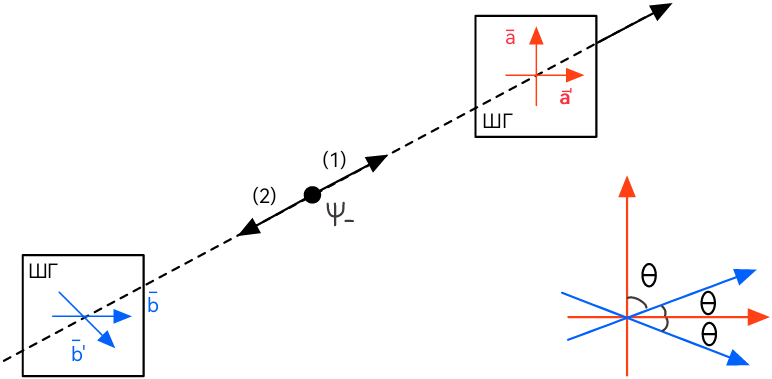
\includegraphics[width=0.75\linewidth]{images/S10_9.png}
	\label{fig:fig1}
\end{figure}

Принимая $\theta = \theta_{ab} = \theta_{a'b}=\theta_{a'b'} = \dfrac{\pi}{4}$, получим
\[
(*) = |3\cos{\dfrac{\pi}{4}} - \cos{\dfrac{3\pi}{4}}| = |4\cos{\dfrac{\pi}{4}}| = 2\sqrt{2}
\]



\subsection{\S X.10 Локальные ящики Попеску-Рорлиха}
Рассмотрим случай, когда $\langle FG\rangle = \langle F'G\rangle = \langle F'G'\rangle = 1$, $\langle FG'\rangle = -1$. Тогда мы получим максимум суммы Белла $\langle S\rangle = 4$. Но, как было показано ранее, ни концепция локального реализма, ни квантовая механика не дотягивают до этого значения. На данный момент не существует теории, описывающей законы физики так, чтобы достичь $max~|\langle S\rangle|$. Но можно задать некий абстрактный закон корреляции, позволяющий математически получить $|\langle S\rangle| = 4$: \textbf{локальные ящики Попеску-Рорлиха}. Опишем их идею.\\

Пусть имеются два черных ящика ($(1)$ и $(2)$), между которыми есть некий, возможно нелокальный, закон корреляции. На вход первому ящику подается классический бит $X = \{0,~1\} = \{F,~F'\}$, на выходе получаем, бит $a=\{0,~1\}$, $(-1)^a = \{-1,~+1\}$ --- значения наблюдаемой. На вход второму ящику подается классический бит $Y = \{0,~1\} = \{G,~G'\}$, на выходе получаем, бит $b=\{0,~1\}$, $(-1)^b = \{-1,~+1\}$ --- значения наблюдаемой.\\

\begin{figure}[H]
	\centering
	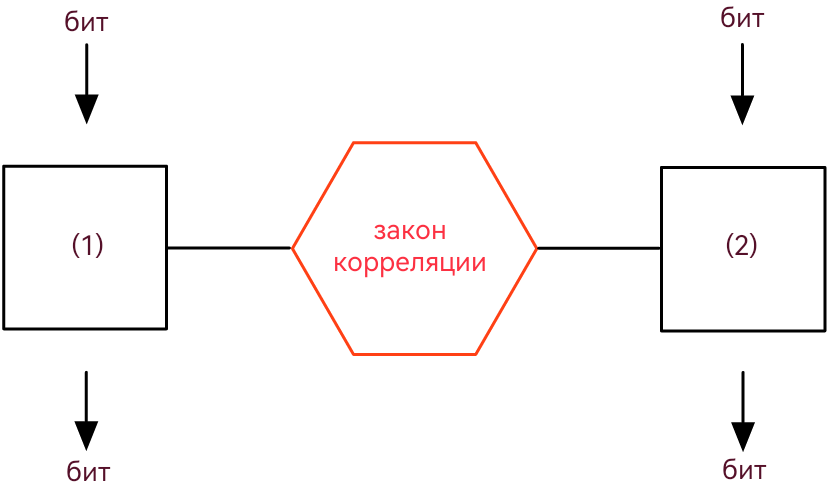
\includegraphics[width=0.75\linewidth]{images/S 10_10.png}
	\label{fig:fig2}
\end{figure}

Эта конструкция описывается вероятностями $w(a,~b~|~X,~Y)$ (16 штук). Пусть теперь ящики удовлетворяют NS-условию:
\[
\sum\limits_{a=0}^1 w(a,~b~|~X,~Y) = w(b~|~Y),\tab \sum\limits_{b=0}^1 w(a,~b~|~X,~Y) = w(a~|~X),
\]
и условию локальности
\[
\forall X=\{0,~1\} \ w(a=0~|~X) = w(a=1~|~X)=\dfrac{1}{2}
\]
\[
\forall Y=\{0,~1\} \ w(b=0~|~Y) = w(b=1~|~Y)=\dfrac{1}{2}
\]
Тогда $\langle FG\rangle$ перейдет в
\[
\langle XY\rangle = \sum\limits_{a=0}^1\sum\limits_{b=0}^1(-1)^a(-1)^b w(a,~b~|~X,~Y)
\]
\[
\Longrightarrow \langle S\rangle = \langle 10\rangle - \langle 11\rangle + \langle 00\rangle + \langle 01 \rangle
\]
Тогда при корреляционном законе $XY = a\oplus b$, где $\oplus$ --- сложение по модулю 2, получим $|\langle S \rangle| = 4$.